\setcounter{chapter}{9}
\chapter{Les Ondes}

\section{Rappels}
\subsection{Onde mécanique progressive ?}

En secouant l'extrémité d'une corde, on observe que la perturbation créée se déplace le long de la corde. Ce phénomène s'appelle la \emph{propagation}. 

Bien que l'onde se propage, la corde ne se déplace pas dans son ensemble. On dit qu'il n'y a pas de transport de matière. 

\blocrouge{Définition}{On appelle onde mécanique, la \trou{propagation d'une perturbation dans un milieu matériel}, sans {transport de matière} et avec transport d'énergie.}



\blocrouge{Définition}{
	\begin{itemize}
%		\item L'\textbf{amplitude} de la déformation caractérise l'écart entre l'équilibre du milieu et la déformation.
		\item La vitesse de propagation $v$ est la vitesse à laquelle se déplace la perturbation. Elle s'exprime en m/s. On l'appelle aussi \textbf{célérité} et on la note parfois $c$.
	\end{itemize}
}

\subsection{Retard d'une onde}

Prenons en photo une corde secouée à deux instants $t$ et $t'$ avec $t<t'$. A l'instant $t$ la perturbation est au point M de la corde. Ensuite la perturbation va toucher d'autres points de la corde en se propageant et M retourne à sa position de repos. A l'instant $t'$, la perturbation a atteint le point $M'$ de la corde.

\begin{center}
	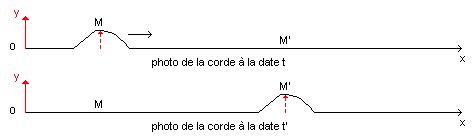
\includegraphics{figures/ondes/retard}
\end{center}

\blocrouge{Vocabulaire}{On appelle retard la durée mise par la perturbation pour aller de $M$ à $M'$ . On dit que le point $M'$ est en \trou{\textbf{retard}} par rapport à $M$. }

\paragraph*{Calcul d'un retard}

On note $d$ la distance entre $M$ et $M'$. On note $\Delta t$ la durée qui s'écoule entre l'instant $t$ et l'instant $t'$. Dans ce cas, la vitesse de l'onde est $$c=\frac{d}{\Delta t}$$ Le retard vaut donc $$\boxed{\trou{\Delta t = \frac{d}{c}}}$$



\section{Ondes progressives périodiques}

Etudier la simulation \url{https://phet.colorado.edu/fr/simulation/wave-on-a-string}
 
\blocrouge{Définitions}{La période temporelle notée $T$ est la plus petite durée, au bout de laquelle, un phénomène se \trou{reproduit identiquement à lui même}. Elle s'exprime en seconde: s.\\
On utilise aussi la fréquence $f$ qui est reliée à la période $T$ selon: $$f=\frac{1}{T}$$ f s'exprime en Hz ou $s^{-1}$.}

 
\paragraph*{Conséquence:}Au bout d'une durée T, tous les points se retrouvent à nouveau dans le même état vibratoire.\\

\subsection{Périodicité spatiale ou longueur d'onde: $\lambda$}
En observant l'onde à un instant $t$ donné, on observe une périodicité tout au long de l'onde. C'est la longueur d'onde: $\lambda$. 

\blocrouge{Définition}{La longueur d'onde $\lambda$ est la plus petite distance entre deux points successifs qui \trou{vibrent en phase} (même état vibratoire à tout instant)}

 C'est aussi la \trou{taille du motif} qui se répète si on observe une photo de l'onde.

\subsection{Relation entre $\lambda$ et $T$}
\begin{center}
	\includegraphics{figures/ondes/fig_relation_propag}
\end{center}

Entre la première et la troisième représentation de l'onde il s'est écoulé une durée égale à T. Pendant ce temps, la perturbation a parcouru une distance égale à $\lambda$ à la vitesse $c$.

\blocrouge{Relation entre période, longueur d'onde et célérité}{$$c=\trou{\frac{\lambda}{T}}$$  
Unités: $\lambda$ en m ; T en s et c en m/s ou \SI{}{\meter\per\second}
}


\section{Le niveau d'intensité sonore}
\subsection{Puissance, intensité, niveau}
Soit une source sonore de puissance P, plus on s'éloigne de la source sonore, plus le son entendu est faible car la puissance sonore se répartit sur une sphère de surface S de plus en plus grande. \\
Donc, on peut poser I l'intensité sonore telle que \begin{center}
\trou{$I=\frac{P}{S}$ }
\end{center}
avec\trou{  P en watts, S en $\si{\meter\squared}$ et I en $\si{\watt\per\meter\squared}$.}
	
	
	\blocrouge{Définition}{
	Le niveau sonore est une grandeur liée à la sensation auditive. Il s'exprime en dB et est défini par la relation : 

	$$\trou{L=10\log\left(\frac{I}{I_0}\right)}$$
$I_0=\SI{e-12}{\watt\per\meter\squared}$ est le seuil d'audibilité.\\
	Par conséquent, on a également 


	$$	\trou{I=I_0\times 10^{L/10}}$$
}

	
	
	\begin{center}
		\includegraphics[scale=0.4]{figures/ondes/fig2.pdf}
	\end{center}


\blocgris{Application}{
Une trompette émet un son dont le niveau sonore vaut : 60 dB. Calculer l'intensité sonore du son de la trompette.\trou{$\SI{e-8}{\watt\per\meter\squared}$}\\ On
fait jouer trois trompettes. Que vaut l'intensité sonore, que vaut le niveau sonore ?\trou{64,8 dB}Conclure sur la linéarité du niveau sonore.\\
Que vaut le rapport : $\frac{I'}{I}$ entre deux sons pour passer de 60 dB à 80 dB ? A combien de trompettes cela correspond-il ? \trou{100}
}

\subsection{Atténuation}
Si l'on s'éloigne de la source sonore ou que l'on place un objet entre la source et notre oreille, le son est atténué. On parle d'atténuation d'un son.
L'atténuation est égale à la différence entre le niveau sonore avant atténuation et le niveau sonore après atténuation.\\
On a donc : \begin{center}
\trou{$A=L_i-L_f$}
\end{center} 
et aussi :\begin{center}
\trou{$A=10 \log\left( \dfrac{I_i}{I_f}\right)$}
\end{center}  avec $I_i$ et $I_f$ les intensités sonores aux instants initiaux et finaux en $\SI{}{\watt\per\meter\squared}$\\
\begin{minipage}{0,7\linewidth}


L'atténuation peut être géométrique, elle est alors due à l'éloignement de la source puisque la surface S sur laquelle se répartit l'onde est de plus en plus grande.\\

L'atténuation peut aussi se faire par absorption, elle est alors due à l'absorption d'une partie de la puissance sonore par un milieu matériel traversé par l'onde.
\end{minipage}
\begin{minipage}{0,3\linewidth}
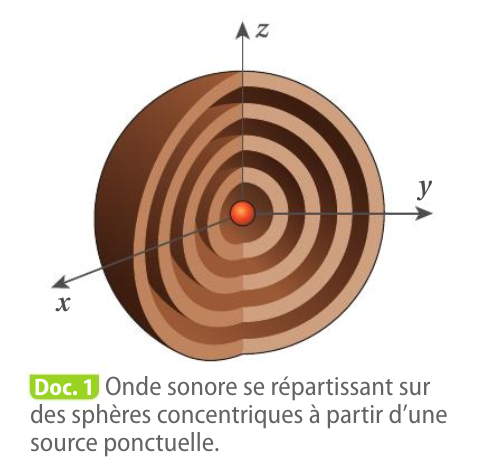
\includegraphics[scale=0.3]{figures/ondes/attenuation.png}
\end{minipage}

\etiquette{Exercices}\\
2,3,7,20 et 21 p 357 et suivantes

\section{Effet Doppler}
\subsection{Présentation}
\blocrouge{Définition}{L'effet Doppler est l'existence d'un décalage entre la fréquence d'une onde émise $f_E$ et la fréquence de l'onde reçue $f_R$ lorsque la distance entre l'émetteur et le récepteur varie.\\ L'écart de fréquence est appelé : décalage Doppler et vaut $\Delta f=f_R-f_E$}

\subsection{Deux situations}
A gauche de la figure, la source est immobile par rapport à l'observateur. Les fronts d'onde sont éloignés de $\lambda$. \\ A droite, l'émetteur se rapproche de l'observateur. La distance entre deux fronts d'onde perçus par l'observateur est plus petite que $\lambda$ donc la fréquence plus grande car $f=c/\lambda$

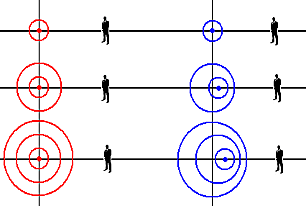
\includegraphics{gfx/Ondes_2012/effet-doppler}

\begin{enumerate}
	\item L'émetteur se rapproche du récepteur alors $f_R>f_E$. \\ Exemple: Lorsque la sirène de l'ambulance se rapproche on perçoit un son plus aigu que lorsque l'ambulance est immobile.
	\item Si l'émetteur s'éloigne du récepteur alors $f_R<f_E$. \\ Exemple: Lorsque la sirène de l'ambulance s'éloigne on perçoit un son plus grave que lorsque l'ambulance est immobile.
\end{enumerate}

\etiquette{Lire p 352}

\etiquetterouge{Démonstration} Livre p 253 et Exercice 24 p 362

\subsection{Application}
L'effet Doppler s'observe aussi bien pour les ondes mécaniques que pour les ondes électromagnétiques. 
\etiquette{Culture}

Les raies du spectre d'une étoile qui s'éloigne de la Terre sont perçues décalées en comparaison avec celles mesurées depuis une source immobile. Ce décalage peut être utilisé pour la mesure d'une vitesse d'éloignement. 
Le décalage vers le rouge des radiations émises par les Galaxies vers la Terre valide l'hypothèse d'un univers en expansion (Les galaxies s'éloignent toutes de la Terre).

L'effet Doppler est aussi utilisé avec des ultrasons pour mesurer la vitesse des globules rouge dans le sang lors d'échographie. 

\etiquette{Exercices}
\begin{itemize}
	\item Ex 10 p 359
	\item Ex 22 p 361
	\item Ex 26 p 263
\end{itemize}
\section{La diffraction} 
\subsection{Observation du phénomène}
\blocgris{Expérience}{
Observation du phénomène de diffraction avec la cuve à onde\\
On place sur le trajet des ondes un obstacle présentant une petite ouverture.\\
On observe \trou{un étalement des directions de propagation de l'onde. L'onde est diffractée}\\
Que se passe-t-il si l'on agrandit l'ouverture ?\\
\trou{le phénomène de diffraction ne s'observe plus}
}

\begin{center}
 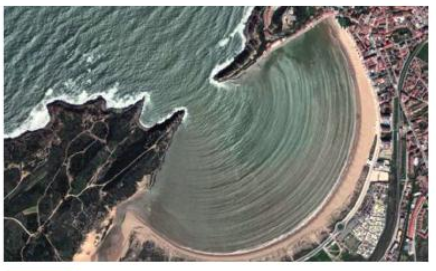
\includegraphics[scale=0.5]{figures/ondes/fig_diff_baie}
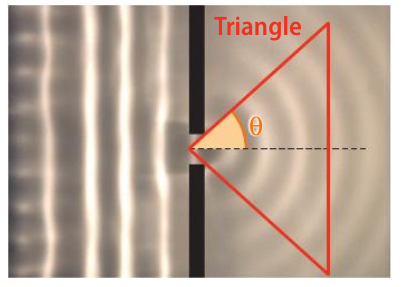
\includegraphics[scale=0.5]{figures/ondes/fig_diff_theta}
\end{center}

On nomme l'angle $\theta$ \textbf{angle caractéristique de diffraction}. Il met en évidence l'importance du phénomène de diffraction.
\blocrouge{Conclusion}{
\trou{
Lorsqu'une onde franchit un obstacle \textbf{de taille comparable ou inférieure à sa longueur d'onde}, on observe un éparpillement de l'onde. On parle de diffraction.
Plus l'ouverture est petite, plus l'angle $\theta$ est grand et plus le phénomène de diffraction est important. }

}

\subsection{Cas des ondes lumineuses}
\blocgris{Expérience}{
Observation du phénomène de diffraction de la lumière\\
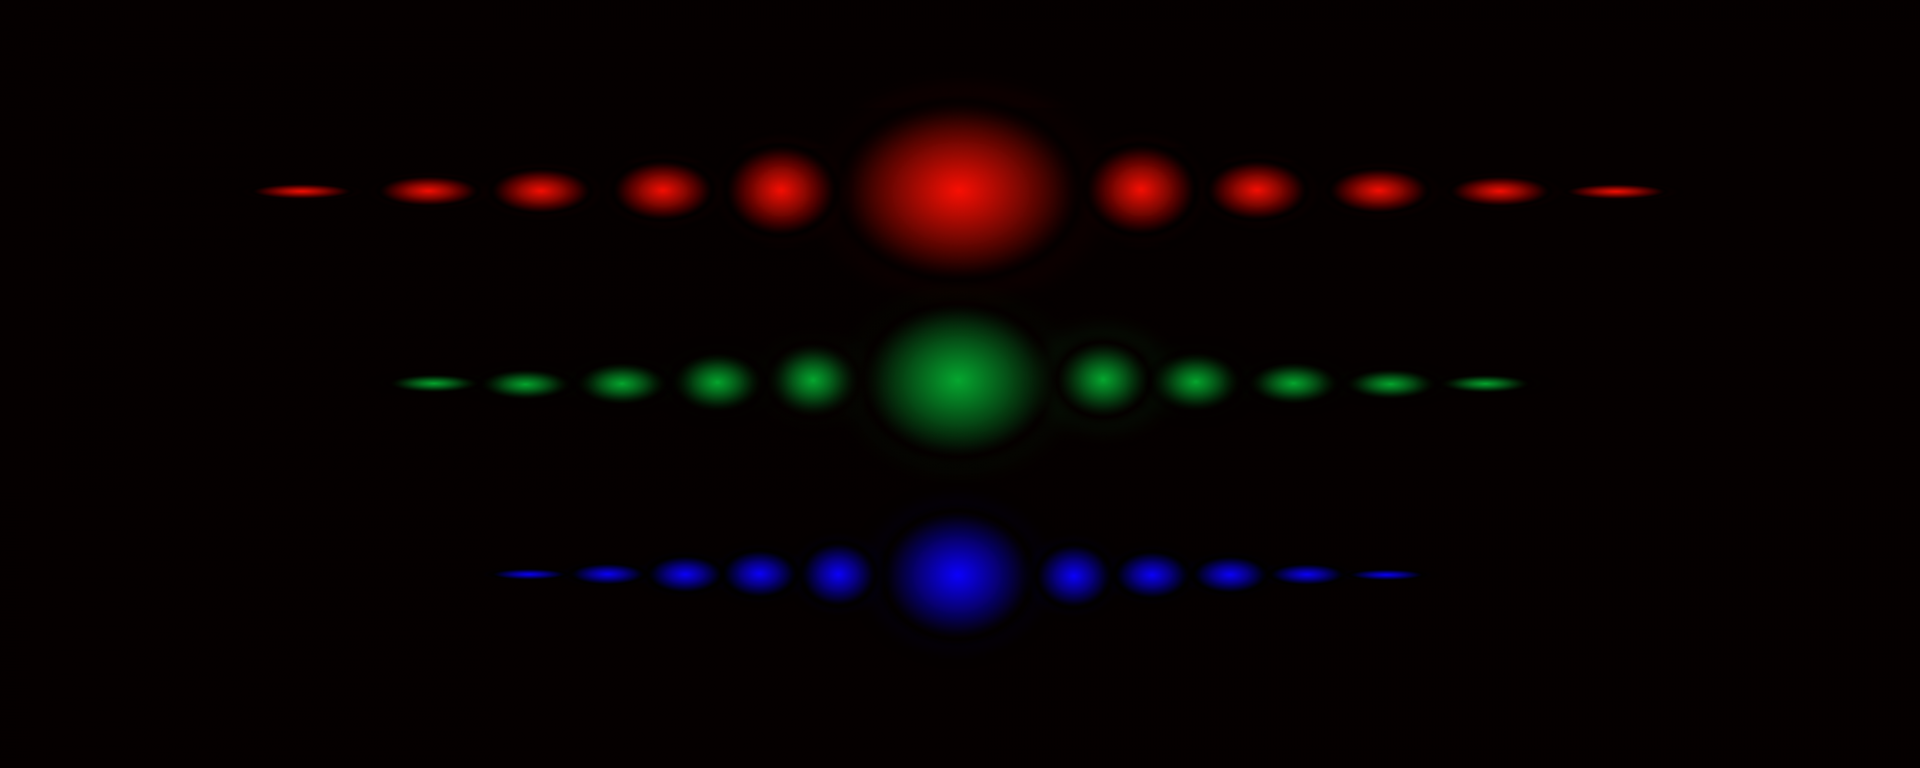
\includegraphics[scale=0.1]{figures/ondes/laser_vert_rouge}
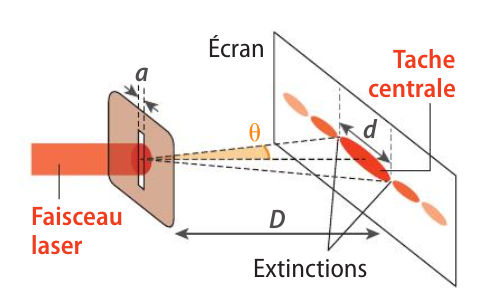
\includegraphics[scale=0.45]{figures/ondes/fig_diff_laser}\\
On place sur le trajet d'un faisceau laser rouge une fente. On réduit peu à peu l'ouverture de la fente.\\
\trou{On observe une alternance de zones lumineuses et sombres. C'est la figure de diffraction.}\\
On remplace le laser rouge ($\lambda = \SI{630}{\nano\meter}$) par un laser vert ($\lambda = \SI{530}{\nano\meter}$). Que constate-t-on ?\\
\trou{On constate que la figure est moins étalée}\\
Quels sont les paramètres influençant la figure de diffraction ?\\
\trou{La largeur de la fente a et la longueur d'onde $\lambda$}\\

}


\etiquette{Application}\\
Parmi les relations suivantes, quelles sont celles qui conviennent après étude des unités ?\\
Quelle est celle qui vous semble conforme aux observations faites ci-dessus ? \\
\begin{center}$\theta=a\times \lambda$ \hspace{2cm}$\theta=\frac{a}{\lambda} $ \hspace{2cm} $\theta=\frac{\lambda}{a}$ \\
\end{center}
\trou{quand a diminue, $\theta$ augmente, et quand $\lambda$ diminue (du rouge au vert), $\theta$ diminue.}
\trou{La relation valable est donc $\theta=\frac{\lambda}{a}$}

\blocrouge{Conclusion}{
\trou{L'écart angulaire $\theta$ est égal à $\frac{\lambda}{a}$ avec $\theta$ en rad, $\lambda$ en m et a en m.}
}


\newpage
\section{Les interférences}

\subsection{Découverte du phénomène}
Considérons un surfeur allongé à l'arrêt sur sa planche. Une vague arrive, le surfeur ne surfe pas, il monte puis redescend et retrouve sa position initiale.\\
Imaginons maintenant qu'une vague arrive d'un côté, et une autre de l'autre côté (peu probable, il est vrai !). deux possibilités : \\
 Les vagues se superposent : Le surfeur monte deux fois plus.
Les vagues s'opposent : Le surfeur ne bouge pas.\\




\verb?http://www.ostralo.net/3_animations/swf/croisement_ondes.swf?\\
Lorsque deux ondes se superposent, leurs élongations s'ajoutent. Deux cas particuliers possibles : \\
\begin{itemize}
\item les deux ondes vibrent en phase

\begin{minipage}{0.5\linewidth}
\centering
\includegraphics[scale=0.3]{figures/ondes/fig2bis}
\end{minipage}
\begin{minipage}{0.5\linewidth}
\centering

\includegraphics{figures/ondes/fig4.pdf}
\end{minipage}
\trou{Dans ce cas, l'amplitude est maximale, on parle d'interférences constructives}
\item les deux ondes sont en opposition de phase\\
\begin{minipage}{0.5\linewidth}
\centering

\includegraphics[scale=0.3]{figures/ondes/fig3}
\end{minipage}
\begin{minipage}{0.5\linewidth}
\centering

\includegraphics{figures/ondes/fig4.pdf}
\end{minipage}
\trou{Dans ce cas, l'amplitude est minimale, on parle d'interférences destructives}
\end{itemize}
C'est ce phénomène qui a lieu dans une cuve à ondes générant deux ondes. Observons-le.\\
\url{https://phet.colorado.edu/sims/html/wave-interference/latest/wave-interference_fr.html}


\vspace{1cm}
\textbf{Analogie pour mieux comprendre :} \\
Imaginons deux personnes qui marchent d'un même pas, des pas de 1m. La longueur d'onde est donc de 2 m pour que le même pied recommence le mouvement.\\
Ces deux personnes doivent poser le pied sur une cible dessinée au sol. On dira que les interférences sont constructives lorsqu'elles posent toutes les deux le même pied, droit ou gauche sur la cible.\\
Elles partent toutes les 2 d'une distance de 4 m, du pied droit, et en même temps.\\
Quel pied vont-elles poser sur la cible ?\\ \trou{Elles vont poser le pied gauche toutes les deux. Interférences constructives.}\\
Maintenant, la personne A ne bouge pas, mais la personne B recule d'un mètre. La personne A a donc 4m à parcourir, mais la personne B doit parcourir 5 m. Quelle est la différence de marche entre les deux personnes, c'est à dire la différence de distance à parcourir ? Que va-t-il se passer ?\\
\vspace{1cm}
\trou{Interférences constructives.}\\

\blocgris{Application}{
\begin{enumerate}
	\item Faire un schéma représentant le chemin parcouru par A et B pour des différences de marche de 2 m, 3 m et 4 m.
	\item Indiquez s'il s'agit d'interférences constructives ou destructives dans chacune des situations. 
	\item Proposez une règle générale pour prédire le type d'interférence à partir de la différence de marche.

\end{enumerate}
}

\vspace{3cm}
En conclusion, on observe que \trou{lorsque la différence de marche est un multiple de $\lambda$, les interférences sont constructives, et que lorsque la différence de marche est un multiple de $\lambda /2$, les interférences sont destructives.}
\\
\blocrouge{Conclusion}{
Dans le cas des interférences constructives : \\
\trou{$\delta= k \times \lambda$ où k est un entier relatif (avec un signe)}\\
Dans le cas des interférences destructives :\\
\trou{$\delta= (k+\frac{1}{2}) \times \lambda$ où k est un entier relatif (avec un signe)}\\
}


\subsection{Interférences lumineuses}

\textbf{cf TP  : Les interférences lumineuses}\\
\etiquette{Vocabulaire} Surligne les mots clés dans le paragraphe suivant:\\
Lorsque deux ondes lumineuses (cohérentes) se superposent, nous observons une figure d'interférences, c'est à dire une alternance de zones brillantes et sombres appelées franges d'interférences.\\
La distance entre 2 franges est appelée interfrange. Elle est notée i. \\
Pour les ondes lumineuses, la différence de marche est aussi appelée différence de chemin optique.

\subsection*{Interférences des trous d'Young : détermination de l'interfrange}

\etiquette{Situation}
Le dispositif des trous d'Young est composé de deux petits trous très proches, ici notés $S_1$ et $S_2$. La distance entre ces trous sera notée b. On éclaire ces trous avec un laser de longueur d'onde $\lambda$, et on place un écran à une distance D très grande devant b.

\begin{minipage}{0.5\linewidth}
\begin{center}
\includegraphics[scale=0.5]{figures/ondes/fig_young.png.pdf}
\end{center}

\end{minipage}
\begin{minipage}{0.5\linewidth}
\begin{center}
\includegraphics[scale=1.3]{figures/ondes/fig_interf}
\end{center}

\end{minipage}


\etiquette{Données du problème}
\begin{itemize}
	\item La longueur d'onde du laser utilisé est égale à $\SI{680}{\nano\meter}$
	\item La distance entre les deux trous, notée b est égale à 0,20 mm.
	\item L'écran sur lequel on observe la figure est placé à 1,20 m des fentes.
\end{itemize}

\etiquetterouge{Objectif} On veut calculer la différence de chemin optique puis l'interfrange $i$ dans le cas d'interférences constructives (puis destructives)
\\
\begin{enumerate}
\item La différence de chemin optique en un point M d'abscisse x est donnée par la relation : \\$\delta=S_2M-S_1M=\dfrac{xb}{D}$ \\

\item Que vaut la différence de chemin optique $\delta$ au centre de la frange centrale ? Est-ce une frange sombre ou lumineuse ?\\
 \trou{$\delta=0$ car le point O est à égale distance des deux sources.}
 
\item Raisonnement avec les franges lumineuses (interférences \trou{constructives}) 
\begin{itemize}
\item Que vaut la différence de chemin optique au centre de la première frange lumineuse ? \trou{$\delta=\lambda$}
\item En déduire la valeur de x au centre de la première frange lumineuse.\\
\trou{$x=\dfrac{\lambda D}{b}$}
\item Sachant que l'interfrange correspond à la distance entre deux franges, déduire la valeur de i.\\
\trou{$i=\dfrac{\lambda D}{b}-0=\dfrac{\lambda D}{b}$}
\end{itemize}

\item Raisonnement avec les franges sombres (interférences \trou{destructives})
\begin{itemize}
\item Que vaut la différence de chemin optique au centre de la première frange sombre ?\\
\trou{$\delta=\dfrac{\lambda}{2}$}
\item En déduire la valeur de x au centre de la première frange sombre ?
\trou{$x=\dfrac{\lambda D}{2b}$}
\item Que vaut la différence de chemin optique au centre de la deuxième frange sombre ?\\
\trou{$\delta=(1+\dfrac{1}{2}) \times \lambda = \dfrac{3\lambda}{2}$}
\item En déduire la valeur de x au centre de la deuxième frange sombre ?\\
\trou{$\dfrac{3\lambda}{2}=\dfrac{xb}{D}$ donc $x=\dfrac{3\lambda D}{2b}$}
\item En déduire la valeur de l'interfrange.\\
\trou{$i=\dfrac{3\lambda D}{2b}-\dfrac{\lambda D}{2b}=\dfrac{2\lambda D}{2b}=\dfrac{\lambda D}{b}$}
\end{itemize}
\item Calculer la valeur de l'interfrange dans les conditions de l'expérience.\\
\trou{$i=\dfrac{\lambda D}{b}=\dfrac{\SI{680e-9}{} \times 1,20}{\SI{0,20e-3}{}}=\SI{4.08e-3}{\meter}=\SI{4.08}{\milli\meter}$}
\end{enumerate}
\underline{remarque }: Pour observer des interférences à partir d'une onde lumineuse il faut créer des sources secondaires à partir de la même source.


\blocrouge{Conclusion}{
Dans une figure d'interférences, les franges brillantes (ou sombres) sont équidistantes. La distance entre 2 franges brillantes (ou sombres) consécutives s'appelle \trou{l'interfrange}. Elle est égale à \trou{$i=\dfrac{\lambda D}{b}$}
}

\etiquette{Exercices} à faire dans votre livre:
\begin{itemize}
\item 2 p 377 ; 
\item 11 p 379 ;
\item  23 p 381 ;
\item  26, 27 p 383 ;
\item Prépa ECE p 385 (à faire absolument pour s'exercer sur la partie diffraction)
\end{itemize}
